% System FSM — Data Glove Review 2, Figure 3
% Compile: pdflatex fsm.tex && pdftoppm -png -r 300 -singlefile fsm.pdf fsm
\documentclass[border=8pt]{standalone}
\usepackage{tikz}
\usetikzlibrary{arrows.meta,positioning,shapes.geometric,calc}
\definecolor{st}{HTML}{E8F0FE}
\definecolor{ft}{HTML}{FDE8E8}
\definecolor{rc}{HTML}{FFF6DA}
\definecolor{edge}{HTML}{333333}
\begin{document}
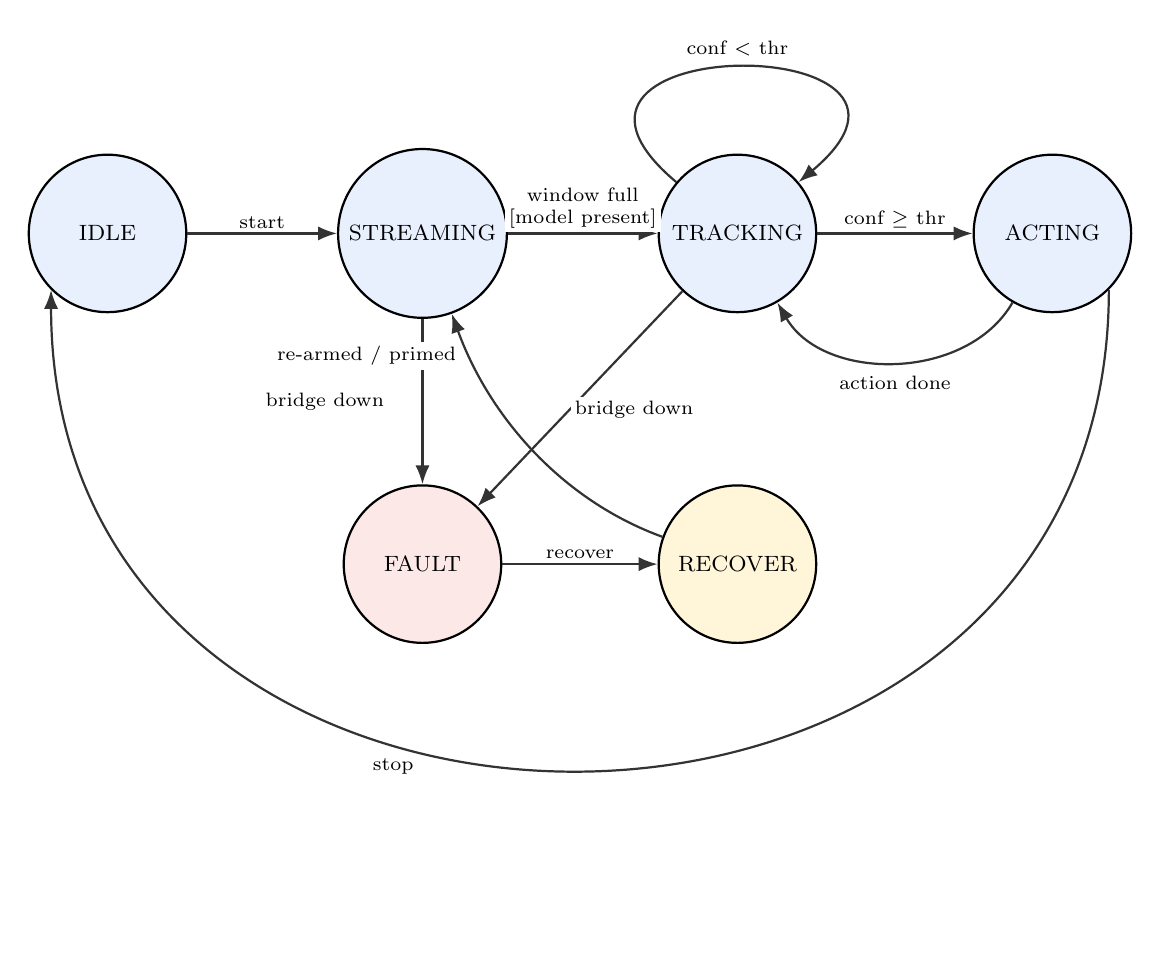
\begin{tikzpicture}[
  font=\footnotesize,
  state/.style={circle, draw, thick, fill=st, minimum size=20mm, align=center},
  fault/.style={circle, draw, thick, fill=ft, minimum size=20mm, align=center},
  rec/.style={circle, draw, thick, fill=rc, minimum size=20mm, align=center},
  tr/.style={-{Latex[length=2.4mm]}, thick, draw=edge},
  lab/.style={font=\scriptsize, fill=white, inner sep=1.5pt, align=center}
]
% ---- explicit grid: x = 0, 4, 8, 12 ; y = 0 (main), -4.2 (fault row) ----
\node[state] (idle)   at (0,0)    {IDLE};
\node[state] (stream) at (4,0)    {STREAMING};
\node[state] (track)  at (8,0)    {TRACKING};
\node[state] (act)    at (12,0)   {ACTING};
\node[fault] (fault)  at (4,-4.2) {FAULT};
\node[rec]   (rec)    at (8,-4.2) {RECOVER};

% ---- happy path (straight, along y=0) ----
\draw[tr] (idle)   -- node[lab, above]{start} (stream);
\draw[tr] (stream) -- node[lab, above]{window full\\{}[model present]} (track);
\draw[tr] (track)  -- node[lab, above]{conf $\ge$ thr} (act);
\draw[tr] (act) to[out=-120, in=-60, looseness=1.0]
  node[lab, below, yshift=-3pt]{action done} (track);
\draw[tr] (track) to[out=140, in=40, looseness=5.0]
  node[lab, above, yshift=2pt]{conf $<$ thr} (track);

% ---- fault + recovery ----
\draw[tr] (stream) -- node[lab, left, pos=0.5, xshift=-12pt]{bridge down} (fault);
\draw[tr] (track)  -- node[lab, right, pos=0.55]{bridge down} (fault);
\draw[tr] (fault)  -- node[lab, above]{recover} (rec);
\draw[tr] (rec) to[out=160, in=-70, looseness=0.9]
  node[lab, left, pos=0.8, xshift=-6pt, yshift=6pt]{re-armed / primed} (stream);

% ---- global STOP: one arc ACTING -> IDLE, hugging the bottom, label on it ----
\draw[tr] (act.south east) to[out=-90, in=-90, looseness=1.55]
  node[lab, below, pos=0.62, yshift=-4pt]{stop} (idle.south west);
\end{tikzpicture}
\end{document}
